\documentclass[final]{article}

\usepackage[paperwidth=48in,paperheight=60in,margin=0in]{geometry}
\usepackage[utf8]{inputenc}
\usepackage[T1]{fontenc}
\usepackage{lmodern}
\usepackage{microtype}
\usepackage{xcolor}
\usepackage{graphicx}
\usepackage{hyperref}
\usepackage{enumitem}
\usepackage{booktabs}
\usepackage{tabularx}
\usepackage{ragged2e}
\usepackage{eso-pic}
\usepackage{tikz}
\setlength{\parindent}{0pt}
\pagestyle{empty}

\definecolor{harvardcrimson}{HTML}{A51C30}
\definecolor{passgreen}{HTML}{2E8540}
\definecolor{failred}{HTML}{B22222}

\newcommand{\overlayblock}[4]{%
  \node[anchor=north west, inner sep=0pt, text width=#3in] at (#1,-#2) {#4};%
}
\newcommand{\posterbody}{\fontsize{15}{19}\selectfont}
\newcommand{\postersmall}{\fontsize{13}{16}\selectfont}
\newcommand{\posterlarge}{\fontsize{24}{28}\selectfont}

\begin{document}
\AddToShipoutPictureBG*{%
  \includegraphics[width=\paperwidth,height=\paperheight,page=1]{SEAS Research Poster 48 x 60 Template.pdf}%
}

% Header region
\begin{tikzpicture}[remember picture,overlay,x=1in,y=1in]
% Mask placeholder text from the template while preserving frame/logo styling.
\fill[white] (12.2,-0.8) rectangle (35.8,-9.2);
\fill[white] (2.4,-14.2) rectangle (15.0,-57.2);
\fill[white] (17.2,-14.2) rectangle (29.8,-57.2);
\fill[white] (32.0,-14.2) rectangle (44.6,-57.2);

\overlayblock{7.0}{1.0}{34.0}{
  \centering
  {\fontsize{54}{58}\selectfont\bfseries\color{harvardcrimson}ROI Tracking in Sports Broadcasts\par}
  \vspace{0.2em}
  {\fontsize{28}{32}\selectfont\itshape Inpaint-First Virtual Advertising for Tennis Court Logos\par}
}
\overlayblock{8.0}{3.0}{32.0}{
  \centering
  {\posterlarge\bfseries
  Enrique Diaz de Leon Hicks \quad Raghav Punnam \quad Giovanni Visi \quad Martina Maiorana\par}
  \vspace{0.2em}
  {\posterbody Harvard SEAS \quad Politecnico di Milano \quad APCOMP 299R Capstone, Spring 2026\par}
  \vspace{0.2em}
  {\postersmall\itshape Advisors: Pavlos Protopapas, Chris Gumb (Harvard), Marco Brambilla (Politecnico di Milano)}
}

% Left column content
\overlayblock{2.2}{13.3}{12.7}{
  \posterbody\justifying
  Tennis broadcasts contain painted ads (for example, the MELBOURNE court logo) that can be replaced with virtual sponsorships. Our goal is to make replacements look physically painted while keeping players naturally in front of the ad.

  We use a software-only, inpaint-first architecture with SAM2.1 segmentation, DiffuEraser cleanup, and MatAnyone 2 alpha matting. This avoids special venue hardware and supports rapid iteration.
}

\overlayblock{2.3}{20.0}{12.6}{
  \posterbody
  \begin{itemize}[leftmargin=1.0em,itemsep=0.3em]
    \item Replace painted court text with new sponsor logos.
    \item Preserve player occlusion with motion-blurred boundaries.
    \item Keep a software-only workflow with cloud GPUs.
    \item Evaluate with objective metrics (jitter, Delta-E, SSIM).
    \item Keep runs reproducible for rapid iteration.
  \end{itemize}
}

\overlayblock{2.5}{33.4}{5.8}{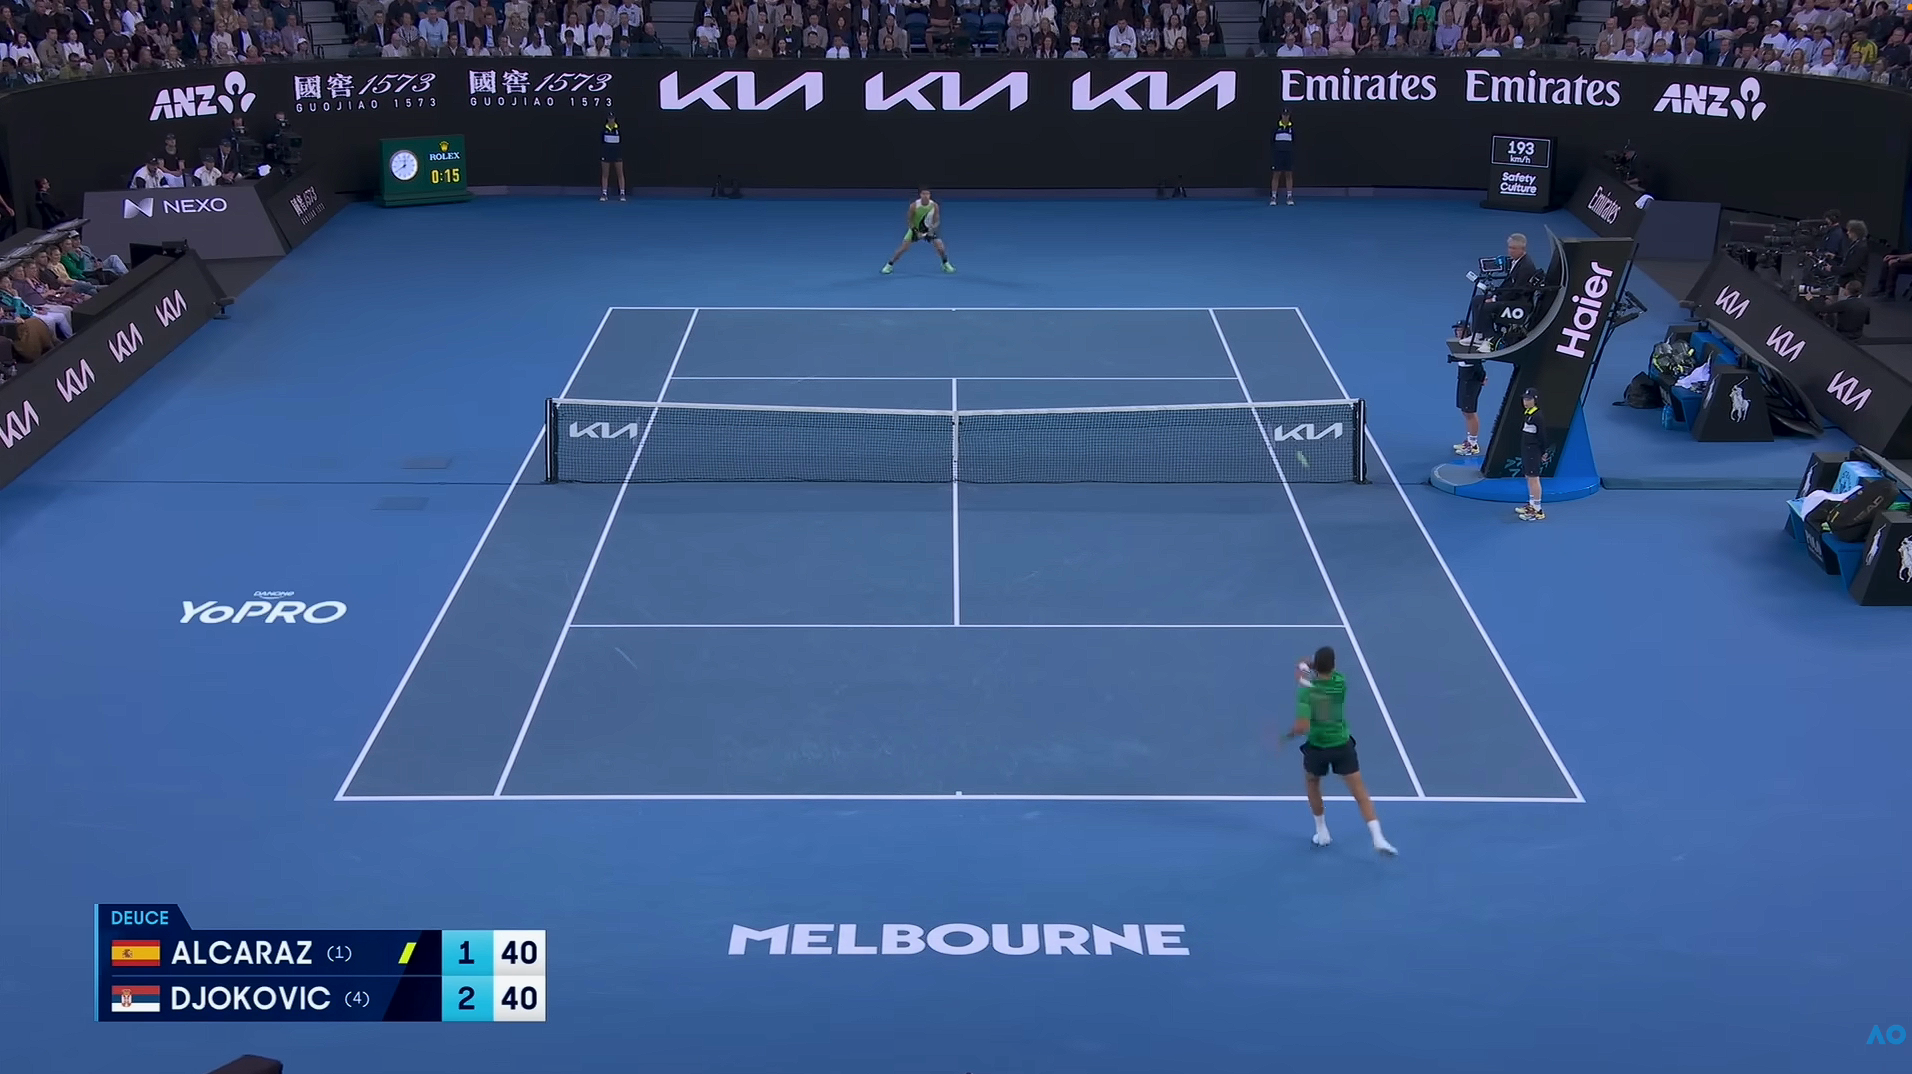
\includegraphics[width=\linewidth]{figures/original_frame_300.png}}
\overlayblock{9.0}{33.4}{5.8}{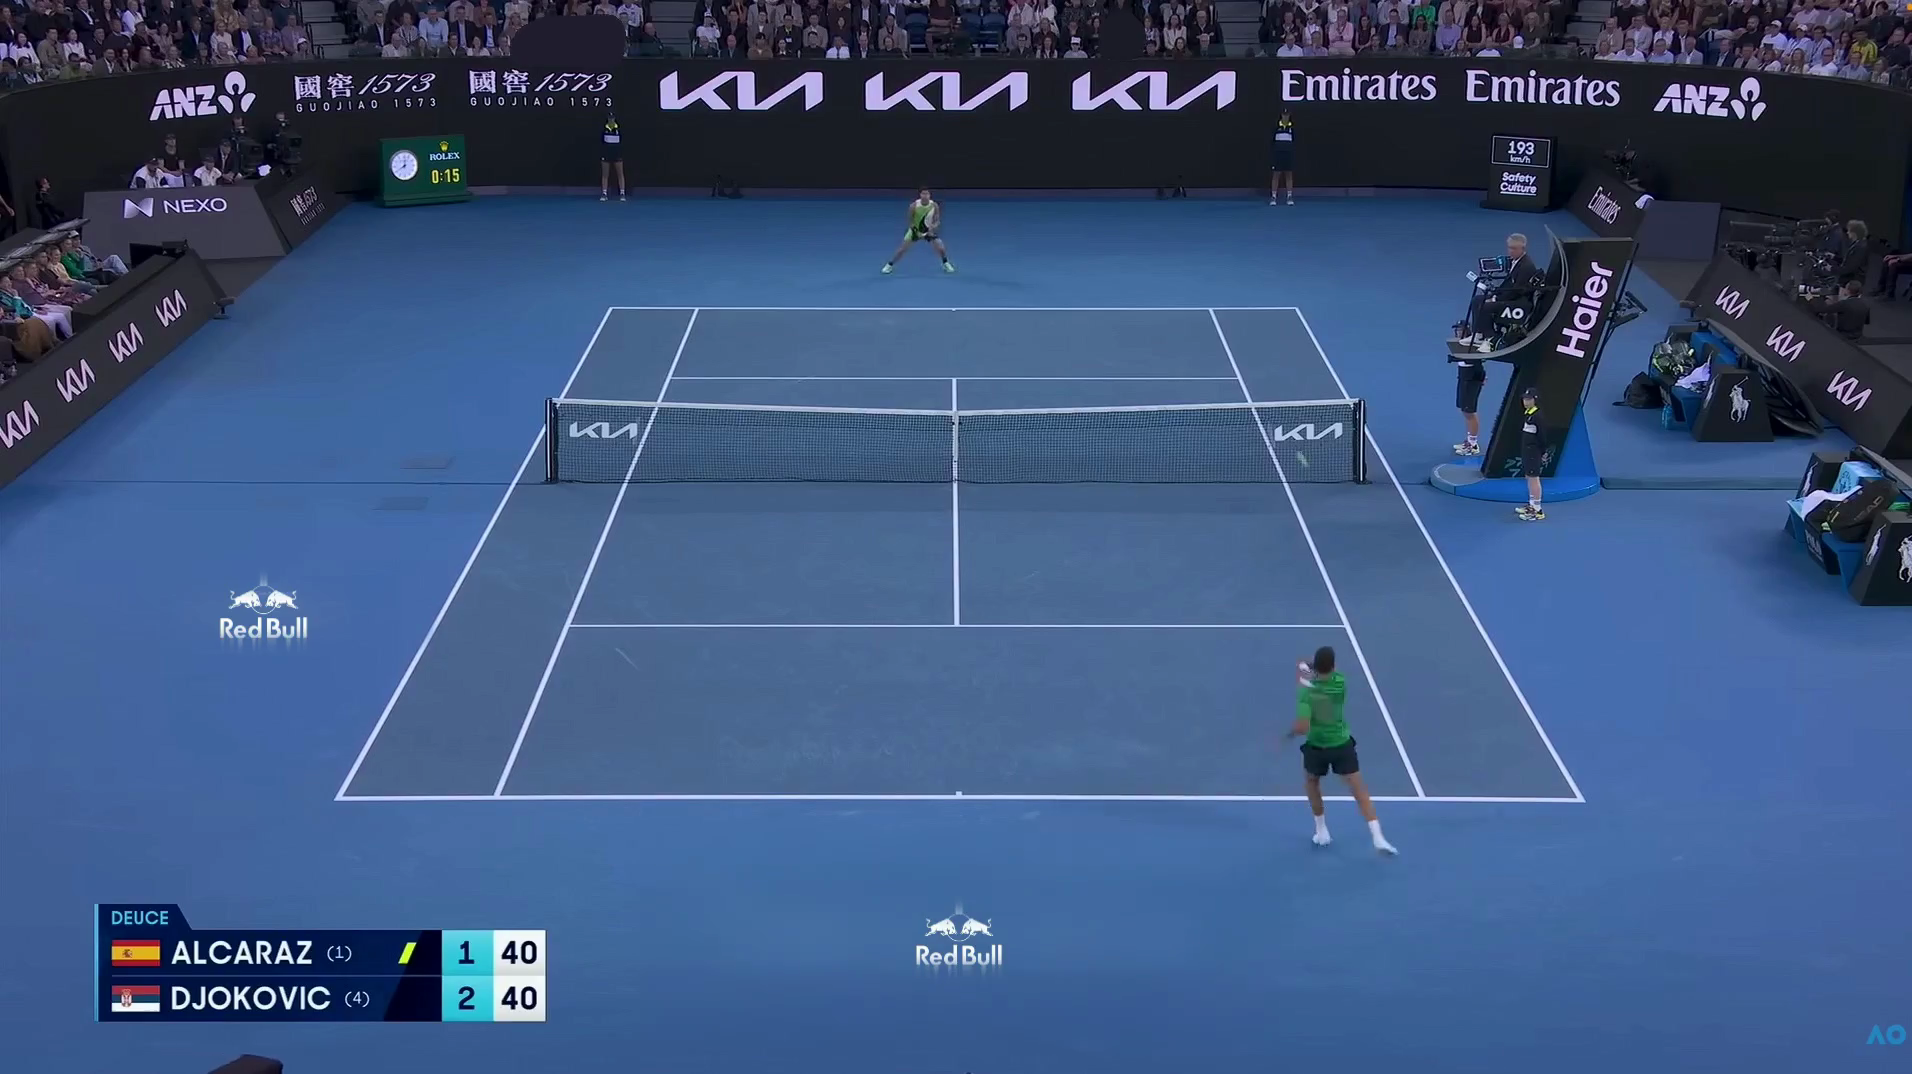
\includegraphics[width=\linewidth]{figures/result_v36_full_300.png}}
\overlayblock{2.5}{40.2}{5.8}{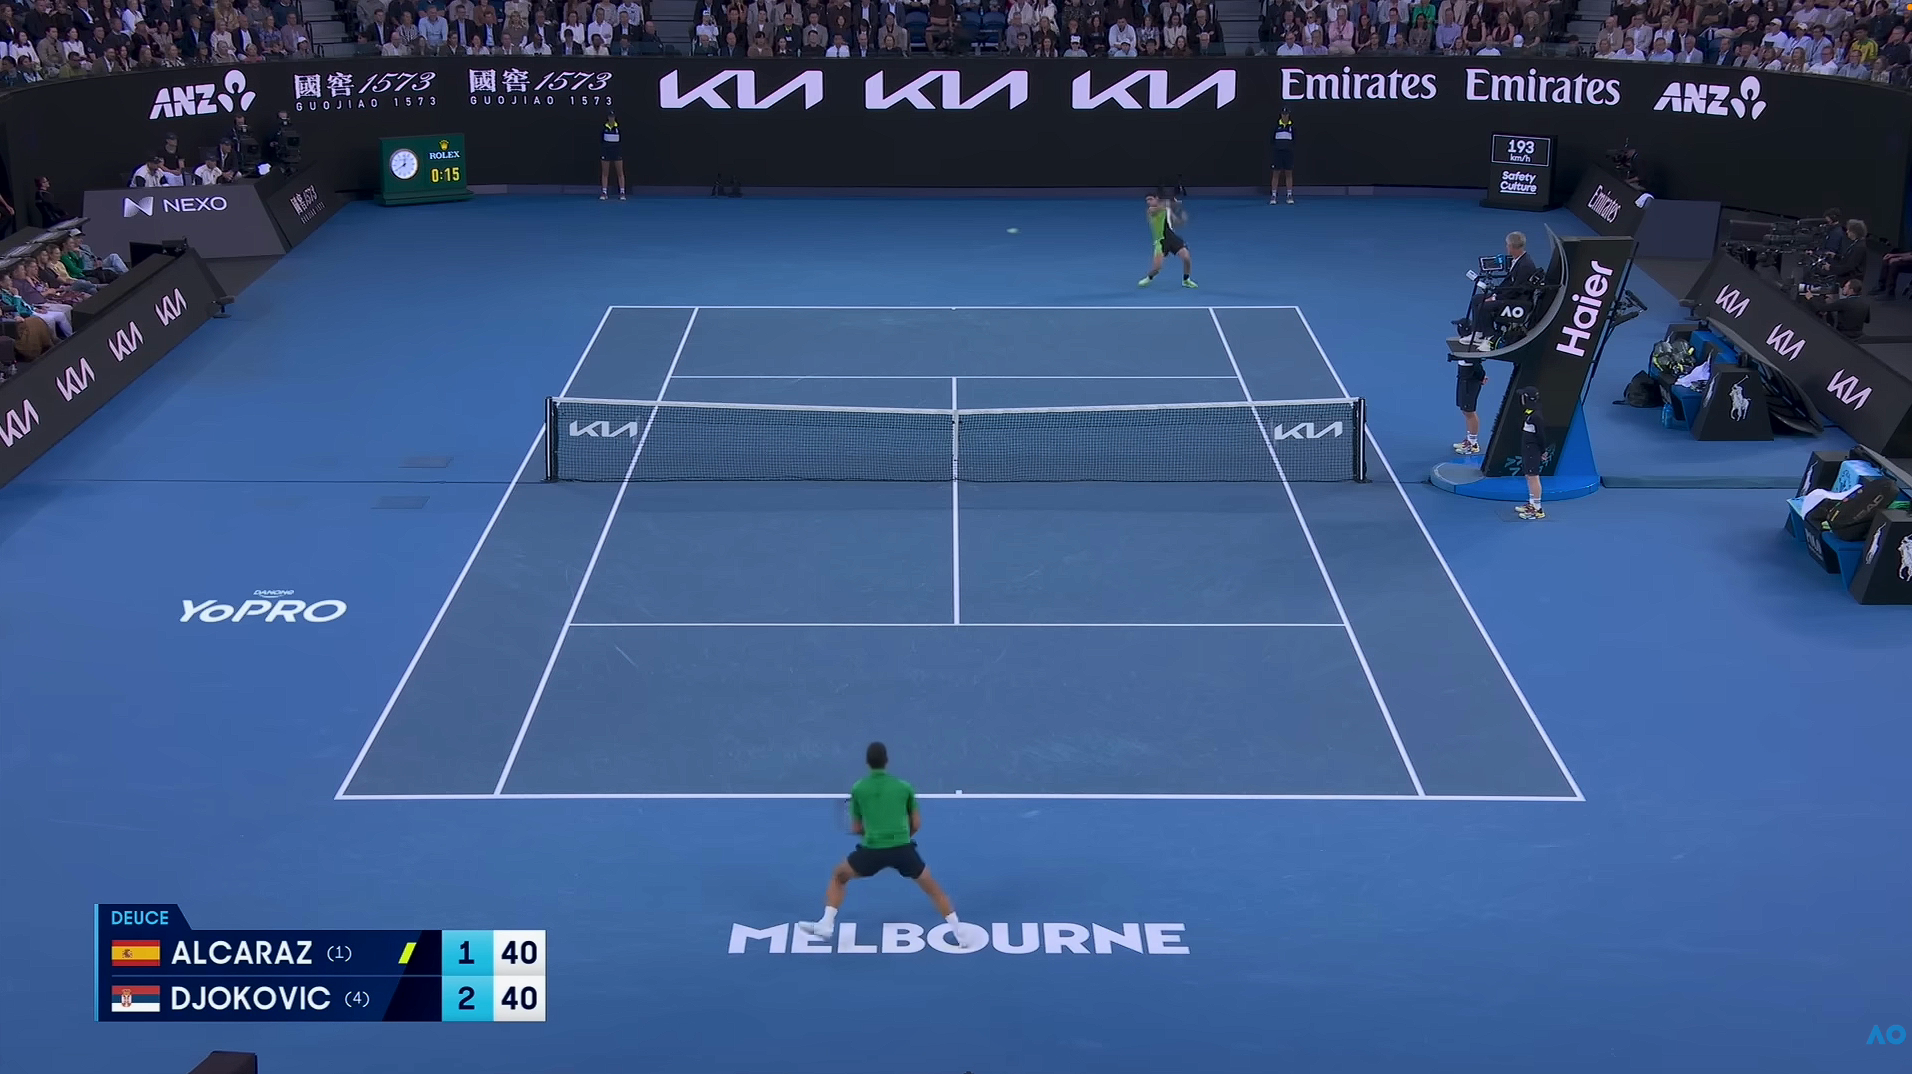
\includegraphics[width=\linewidth]{figures/original_frame_700.png}}
\overlayblock{9.0}{40.2}{5.8}{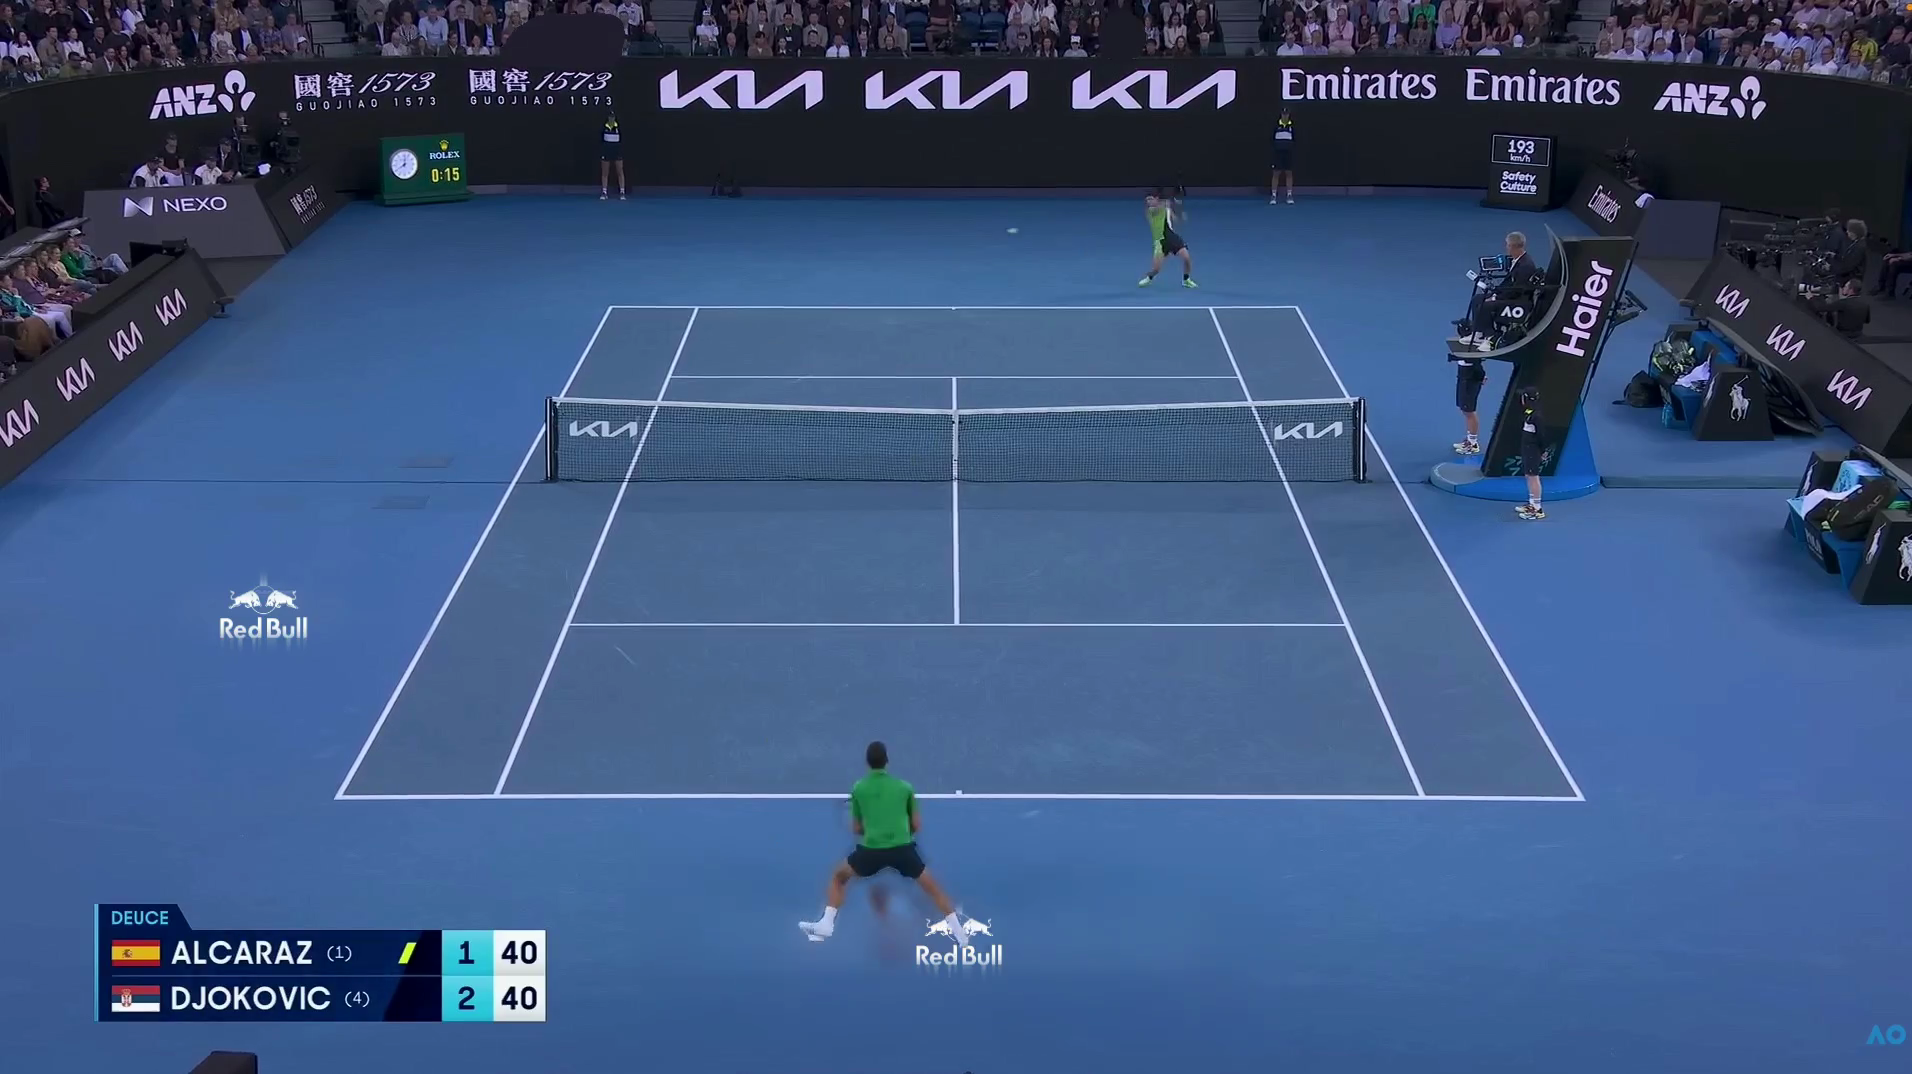
\includegraphics[width=\linewidth]{figures/result_v36_full_700.png}}
\overlayblock{2.3}{47.0}{12.4}{\postersmall\centering Frame comparison from the walking clip. The replacement remains stable while preserving player occlusion.}

% Middle column content
\overlayblock{17.3}{13.3}{12.5}{
  \posterbody\justifying
  \textbf{Methods.}
  The system runs in two offline passes on Modal GPUs. Pass 1 segments players with SAM2.1 and builds a player-aware inpaint mask (court area intersected with NOT player mask). DiffuEraser then removes painted text.

  Pass 2 composites sponsor graphics using luminance matching, outlier cleanup, homography warp, and MatAnyone 2 soft alpha blending.
}

\overlayblock{18.2}{18.8}{10.8}{
  \posterbody
  \begin{enumerate}[leftmargin=1.2em,itemsep=0.2em]
    \item Player segmentation (Mask R-CNN + SAM2.1 propagation).
    \item Player-aware inpaint mask generation.
    \item DiffuEraser clean video creation.
    \item Luminance restoration + cleanup.
    \item Homography warp + alpha blend.
  \end{enumerate}
}

\overlayblock{17.8}{25.0}{3.0}{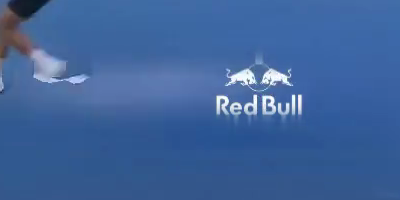
\includegraphics[width=\linewidth]{figures/evo_v7_foot.png}}
\overlayblock{20.8}{25.0}{3.0}{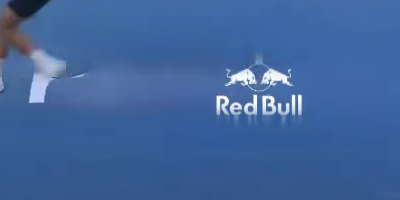
\includegraphics[width=\linewidth]{figures/evo_v12_foot.png}}
\overlayblock{23.8}{25.0}{3.0}{
\includegraphics[width=\linewidth]{figures/evo_v33_foot.png}}
\overlayblock{26.8}{25.0}{3.0}{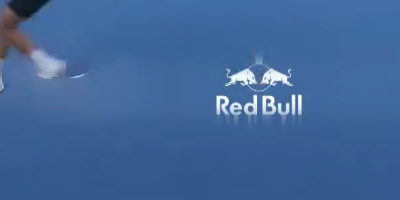
\includegraphics[width=\linewidth]{figures/evo_v36_foot.png}}
\overlayblock{17.3}{28.4}{12.3}{
  \postersmall\justifying
  Evolution crop (same frame area): v7 ghost-leg smear, v12 shadow artifacts, v33 white wedge, v36 clean edge with MatAnyone 2.
}

\overlayblock{17.5}{31.0}{12.0}{
  \posterbody
  \begin{tabularx}{\linewidth}{@{}lXcc@{}}
  \toprule
  \textbf{Metric} & \textbf{Value} & \textbf{Threshold} & \\
  \midrule
  Jitter ratio & 0.6716 & $\leq 1.05$ & \textcolor{passgreen}{\textbf{PASS}} \\
  Inpaint color Delta-E & 1.529 & $< 5.0$ & \textcolor{passgreen}{\textbf{PASS}} \\
  Temporal SSIM & 0.9993 & $> 0.95$ & \textcolor{passgreen}{\textbf{PASS}} \\
  Corner max jump (px) & 413.6 & $< 2.0$ & \textcolor{failred}{\textbf{FAIL}} \\
  Logo area CV & 0.1035 & $< 0.05$ & \textcolor{failred}{\textbf{FAIL}} \\
  Overlay accel p95 (px) & 412.0 & $< 1.0$ & \textcolor{failred}{\textbf{FAIL}} \\
  \bottomrule
  \end{tabularx}
}
\overlayblock{17.3}{36.8}{12.3}{\postersmall\justifying Photometric metrics pass strongly; geometric stability remains the primary remaining engineering target.}

% Right column content
\overlayblock{32.3}{13.2}{12.6}{
  \posterbody
  \begin{enumerate}[leftmargin=1.2em,itemsep=0.35em]
    \item Static masks fail because temporal inpainting can restore removed text.
    \item Player-aware dynamic masks are required for robust results.
    \item DiffuEraser removes text more aggressively than ProPainter, but needs cleanup.
    \item MatAnyone 2 improves motion-edge quality over binary compositing and over MatAnyone v1.
    \item Quad-edge feather plus luminance matching are essential for realism.
  \end{enumerate}
}

\overlayblock{32.3}{20.4}{12.6}{
  \posterbody
  \begin{itemize}[leftmargin=1.0em,itemsep=0.35em]
    \item Replace black KIA back-banner regions with new sponsors.
    \item Improve side-line logo perspective correction.
    \item Reduce corner-jump and logo-area-variance instability.
    \item Re-validate on zoom and broader clips.
    \item Move from offline cloud processing toward real-time.
  \end{itemize}
}

\overlayblock{32.3}{27.2}{12.6}{
  \posterbody
  \begin{itemize}[leftmargin=1.0em,itemsep=0.3em]
    \item Modal H200/B200 GPUs with cached checkpoints.
    \item Reproducible experiment folders with config, metrics, and output videos.
    \item Current best config: eval\_walkover\_inpaint\_first\_v36.yaml.
  \end{itemize}
}

\overlayblock{32.3}{32.2}{12.6}{
  \postersmall
  [1] Ravi et al., SAM2, 2024.\par
  [2] Yang et al., MatAnyone, CVPR 2025.\par
  [3] Yang et al., MatAnyone 2, CVPR 2026.\par
  [4] Zhou et al., ProPainter, ICCV 2023.\par
  [5] Li et al., DiffuEraser, 2025.\par
  [6] He et al., Mask R-CNN, ICCV 2017.
}

\overlayblock{32.3}{38.8}{12.6}{
  \posterbody
  Enrique Diaz de Leon Hicks --- Harvard SEAS \\
  Raghav Punnam --- Harvard SEAS \\
  Giovanni Visi --- Politecnico di Milano \\
  Martina Maiorana --- Politecnico di Milano \\
  \vspace{0.2em}
  \postersmall
  Advisors: Pavlos Protopapas, Chris Gumb, Marco Brambilla \\
  Repo: capstone-data-candidates/homography-fitting
}
\end{tikzpicture}

\end{document}
